\documentclass[10pt]{article}
\usepackage{setspace}
\usepackage{amsmath,amssymb, amsthm}
\usepackage{graphicx}
\usepackage{bm}
\usepackage[hang, flushmargin]{footmisc}
\usepackage[colorlinks=true]{hyperref}
\usepackage[nameinlink]{cleveref}
\usepackage{footnotebackref}
\usepackage{url}
\usepackage{listings}
\usepackage[most]{tcolorbox}
\usepackage{inconsolata}
\usepackage[papersize={8.5in,11in}, total={6in, 9.5in}]{geometry}
\usepackage{float}
\usepackage{caption}
\usepackage{esint}
\usepackage{url}
\usepackage{enumitem}
\usepackage{subfig}
\usepackage{wasysym}
\newcommand{\inlinecode}{\texttt}

\usepackage{etoolbox}
\patchcmd{\thebibliography}{\section*{\refname}}{}{}{}


\begin{document}
\linespread{1}


\title{\textbf{A Brief Introduction of checkm8} \\
        \large \textbf{-- an unpatchable iOS jailbreaking method\\}}

\author{Shaochen (Henry) ZHONG}
\date{Due on December 6; submitted on December 4, 2019\\EECS 338, Dr. Ronald Loui}
\maketitle

\begin{abstract}
    \inlinecode{checkm8} is a recently released (Sep 27, 2019) jailbreaking tool developed by \inlinecode{axi0mX}. Being a jailbreak method targeting the BootROM (a.k.a \inlinecode{SecureROM}) of iOS devices, it is well-known for its unpatchable nature and strong compatibility across 11 generations of iOS devices. This article is intended to give a brief introduction of \inlinecode{checkm8}, with a proper exposure of knowledge from the very concepts and needs of iOS jailbreaking, to the highlighted characters of \inlinecode{checkm8}, then to provide a relatively more technical walk-through on the hacking mechanism implemented in \inlinecode{checkm8}. In the end, it analyzes the philosophical reason behind this exploitation and provides some potential solutions to prevent it from happening again.
\end{abstract}





\vspace{0.5cm}
{\hypersetup{hidelinks}
\tableofcontents
}


\newpage

\section{Jailbreaking under the iOS context}

Jailbreaking -- under the context of iOS -- is an act of gaining superuser access of Apple's mobile/tablet operating system(s). Since Apple restricts such superuser privilege by default, a successful jailbreak is typically performed with exploitations of bugs and system design flaws, known as \textit{privilege escalation}.

Throughout the history of iOS jailbreaking, there are various successful -- or semi-successful -- jailbreak methods; and the capability of each jailbreak method also varies depending on its attack methodology and Apple's patch. However, the main and common goals of all jailbreak methods are the same: to bypass the software installation restrictions imposed by Apple; and to utilize previously unavailable lower level portals (e.g., APIs) to collect data and therefore develop features that are impossible to implement under a non-jailbroken device.

\section{\inlinecode{checkm8}: the overview}

Like many other releases of jailbreaking tools, \inlinecode{checkm8} is a recently released (Sep 27, 2019) jailbreaking tool developed by \inlinecode{axi0mX} \cite{cite:2}. While each successful jailbreak method has its pros and cons, the highlights of \inlinecode{checkm8} are:
\begin{itemize}
    \item It is unpatchable by the nature of the BootROM exploitation, meaning that Apple will never be able to release a patch to invalid the tool.
    \item It is applicable to a vast generation of iOS devices, from iPhone 4s (A5 chip) to iPhone 8/X (A11 chip). This means millions of active devices in use today can benefit or be targeted by this jailbreaking method.
\end{itemize}

\subsection{The unpatchable nature}

\inlinecode{checkm8} targets the BootROM (a.k.a \inlinecode{SecureROM}) of iOS devices -- which is a low-level read-only ROM that being utilized during the booting stage of iOS devices. With the bugs that \inlinecode{checkm8} exploits and proper implementation of Heap Feng-shui\footnote{Details refer to \textit{Section 3.3 iBoot and Heap Feng-shui.}}, you can execute any code at the BootROM level, thus carry out a successful jailbreak.

Due to the read-only nature of BootROM, the booting code is encoded in a hardware manner when a device is manufactured. Thus it is impossible for Apple to release software security patches to alter the code within BootROM, and therefore results in an unpatchable hack. Also, since a vast amount of iOS devices share BootROMs with similar architecture, the compatibility of a BootROM exploitation can be simultaneously widely applicable and long-standing.

\subsection{The lack of persistence}

Though with many highlights, one significant limitation of \inlinecode{checkm8} is its lack of persistence. Since to the mechanism of \inlinecode{checkm8} is to exploit the BootROM -- which is essentially a type of ROM -- a jailbroken device will back to its unexploited state once a reboot is performed. Thus making \inlinecode{checkm8} only a tethered jailbreak\footnote{The term `tethered jailbreak' is the antonym of `untethered jailbreak,' where the latter one refers to jailbreak methods which are so powerful that they can exploit a device even after rebooting, and without the aid of a connected computer.}. In a real-life scenario, a solo\footnote{\inlinecode{axi0mX} admits that it is theoretically possible to remotely jailbreaks -- thus `hacks' -- a \inlinecode{checkm8} supported device by using a chain of exploits that available and unavailable to the public \cite{cite:3}. However, it is extremely unlikely to happen due to the technical mechanism of \inlinecode{checkm8} and the mindset of malicious attackers. More about it in \textit{Section 2.3 The potential of malicious uses}.}\inlinecode{checkm8} jailbreak is only possible by turning the phone into DFU (Device Firmware Upgrade) mode and connect it to a computer (to run scripts that inject custom code) .

\subsection{The potential of malicious uses}
\subsubsection{The protection of Secure Enclave}
One of the major concerns of \inlinecode{checkm8} is the fear of privacy breaches due to the implementation of \inlinecode{checkm8}. According to \inlinecode{axi0mX}, devices with the feature of Secure Enclave\footnote{Secure Enclave is a security feature implemented with a separately booted 4MB flashable AKF processor core called the secure enclave processor (SEP). It performs biometric checks and decrypts the information -- thus, the main operating system will not directly read the encryption key stored in Secure Enclave's storage. It is only implemented within devices that have A7 chip or later (with Touch ID or Face ID).} will protect your data if the possessor of your phone cannot input the correct credential; as it is stored in a separate system, and \inlinecode{checkm8} is not effective to the secure enclave processor. However, for devices with no Secure Enclave feature, the data within such a device can be easily compromised as there is no separate system protecting it \cite{cite:3}.

Note that \inlinecode{axi0mX} also mentions the fact that accessing the data of a device is likely not the only goal for an attacker \cite{cite:3}. Thus although your data can be protected with Secure Enclave, the attacker might be going after something else -- e.g., reselling the phone with a ``seemingly fresh" system.

\subsubsection{Unencourage factors to attackers with malicious intents}
In \textit{Section 2.2}, I have introduced the fact that for one to perform a \inlinecode{checkm8} jailbreak, it is required to obtain physical access of the phone and connect to a computer with proper tools installed and scripts available. Thus, \inlinecode{checkm8} cannot be performed remotely by nature. \inlinecode{axi0mX} also emphasizes the idea that it is unlikely that \inlinecode{checkm8} will be vastly used for malicious purposes, as most attackers with malicious intents prefer to stay in the distance -- e.g., utilizing phishing emails, webpages, Wi-Fi hotspots, etc. -- but not to be physically up-clos \cite{cite:3}. While \inlinecode{checkm8}'s nature of requiring physical access makes close physical contact inevitable, and thus likely not preferred by malicious attackers.

\section{\inlinecode{checkm8}: the mechanism}
\subsection{The booting mechanism of iOS}

To establish a minimum understanding of \inlinecode{checkm8}, it is required to have a proper explosure to the booting mechanism of iOS devices. It is demonstrated as [\figurename{ \ref{figure_1}}].
\begin{figure}[!ht]
    \centering
    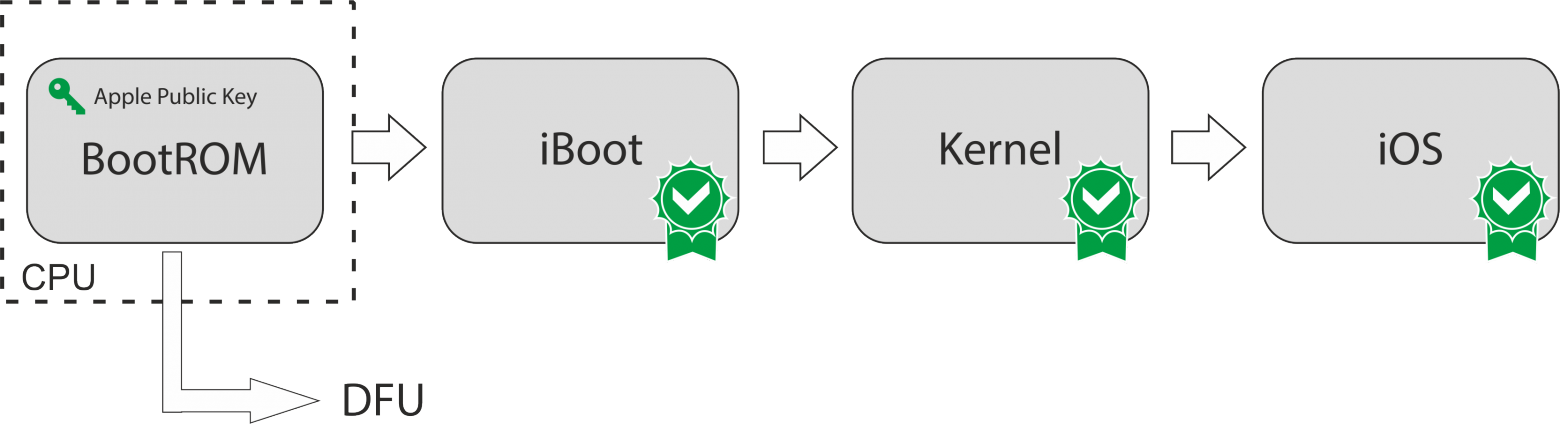
\includegraphics[width = 0.6\textwidth]{figure_1}
    \caption{The Secure Boot Chain of iOS \protect\cite{cite:4}}
    \label{figure_1}
\end{figure}

The \inlinecode{Kernel} and \inlinecode{iOS} stages are rather self-explanatory, while the \inlinecode{BootROM} and \inlinecode{iBoot} are not. In short, every stage will perform its task, check for the integrity of the system, and load and prepare to move to the next stage. Thus, \inlinecode{BootROM} is responsible for executing the first several programs of the booting, checking the integrity, and loading necessary data to prepare for moving to the \inlinecode{iBoot} stage. Then \inlinecode{iBoot} does the same for \inlinecode{Kernel} stage. Note that due to the similar in functionalities, \inlinecode{BootROM} shares a significant amount of system and library code with \inlinecode{iBoot} \cite{cite:4}.

As introduced in \textit{Section 2.1}, \inlinecode{BootROM} is a read-only memory with code encoded in a hardware manner when a device is manufactured; thus, it has the character of unwritable (and therefore unpatchable). Apple further implements security protocol to lock its memory storage once all executions within the \inlinecode{BootROM} stage are completed \cite{cite:4}\cite{cite:1}; thus, it \textbf{should} also be unreadable to users.

\subsection{Exploiting \inlinecode{SecureROM} under DFU mode}

Apple's philosophy is, if a program is unwritable and unreadable, then it is certainly safe. However, \inlinecode{checkm8} manages to exploit a design flaw under the Device Firmware Upgrade mode\footnote{DFU is part of the \inlinecode{BootROM}. It is designed to restore a device by running a temporary system from USB.} of the devices. For the sake of readability, here is a simplified version\footnote{Infomation regarding \inlinecode{wLength} data length check, \inlinecode{stall, leak, no\_leak} asynchronous execution, and details regarding DFU main/interface code are intentionally left out for simplification \cite{cite:4}.} of the procedure of DFU mode \cite{cite:4}\cite{cite:1}\cite{cite:5}:

\begin{enumerate}
    \item \inlinecode{usb\_dfu\_init()} is called, an command-handling interface is registred and a buffer is allocated (hereinafter \inlinecode{io\_buffer}).
    \item Send a \inlinecode{DFU\_DNLOAD} request that eventually calls out to the interface code.
    \item DFU checks the request package, if the request package is shorter than the allocated \inlinecode{io\_buffer}, the pointer to \inlinecode{io\_buffer} is passed to a global variable.
    \item The request package is copied into the \inlinecode{io\_buffer}.
    \item DFU stores the \inlinecode{io\_buffer} into a device-specific address for loading the operating system.
    \item The USB code will reset all variables (including the global variable containing \inlinecode{io\_buffer}) and ready to handle the new package.
    \item Once all packages are handled, a \inlinecode{DFU\_DONE} request will be sent, and DFU will therefore free the \inlinecode{io\_buffer}), and then try to boot device with the system stored at the device-specific address. If the boot is a success then you enter the temporary OS; otherwise, \inlinecode{usb\_dfu\_init()} is called again, and the device is back to the first stage.
\end{enumerate}

The bug is embedded in \textit{Step 3} and \textit{Step 7}. As you may send a \inlinecode{DFU\_DONE} request\footnote{By modifying the USB controller \cite{cite:5}.} at \textit{Step 3} to bypass \textit{Step 4} to \textit{Step 6}. Altough the \inlinecode{io\_buffer} is freed in \textit{Step 7}, the global variable updated in \textit{Step 3} still points to the supposely freed \inlinecode{io\_buffer}, therefore results a \textit{use-after-free} scenario \cite{cite:1}\cite{cite:5}.

\subsection{iBoot and Heap Feng-shui}
\inlinecode{checkm8} exploits the \textit{use-after-free} flaw by taking several spots on the heap. As the \inlinecode{SecureROM} of iOS uses \inlinecode{libc} version of \inlinecode{malloc()}, it is possible to induce some critical requests to store at the address of \inlinecode{io\_buffer} which we have access of -- this kind of maneuver is known as \textit{heap feng-shui}. Then, by altering the value within \inlinecode{io\_buffer}, we may complete a jailbreak \cite{cite:1}.

Note this is an oversimplification of what \inlinecode{checkm8} does. \inlinecode{checkm8} utilizes the \inlinecode{usb\_device\_io\_request} structure to construct a \inlinecode{callback-chain}, and eventually gets the device to execute the exploit's payload stored in \inlinecode{io\_buffer} \cite{cite:4}. \inlinecode{checkm8} also relies on the leaked \inlinecode{iBoot} source code to reverse-engineer the addresses of many functions within \inlinecode{BootROM} -- as the \inlinecode{iBoot} code is vastly shared with the \inlinecode{BootROM} \cite{cite:4}\cite{cite:1}.


\section{Summary}
In summary, the philosophy of relying on confidentiality to protect system security is a rather unrestful idea \cite{cite:1}. As code and manual can be leaked by human -- in this case, the leaking of \inlinecode{iBoot} is the initial cause of this catastrophic security breach -- and the manufacture will not be able to refactor as the code is already in ROM. Instead, a comprehensive testing procedure should be enforced -- e.g., fuzz testing -- to ensure the security completeness of the program.

However, the overhead of building a testing procedure that is comprehensive enough is considerably huge; meanwhile the creativity of hackers can never be underestimated. Thus, a commonly embraced soluition is transparency: e.g., invites hackers to security contests, or even open-sourcing the code for public scrutiny. By doing that, the manufacture may actively refactor its code based on public (e.g., whitehat community) feedback. And most importantly, the objective quality of product can be therefore improved as it is now ``more secured,'' instead of ``secured if kept confidential.''


\newpage
\section{References}

\nocite{*}
\raggedright
\bibliography{references.bib}
\bibliographystyle{plain}


\end{document}